\documentclass[a4paper,10pt]{article}
\usepackage[utf8]{inputenc}
\usepackage{graphicx}
\usepackage{hyperref}
\usepackage{geometry}
\usepackage{listings}
\usepackage{algorithm}
\usepackage{algorithmic}
\usepackage{caption}
\usepackage{subcaption}
\usepackage{fancyhdr} 
\pagestyle{fancy}
\usepackage[enabled,section]{easy-todo}
\usepackage{lscape}
\def\UrlBreaks{\do\/\do-}

\geometry{hmargin=2.5cm,vmargin=1.5cm}
%opening
\title{eHECOPS - Enhanced Localization Algorithm for WSNs}
\author{ Thibault Rihet\\
Software/Hardware Integration Lab\\
Federal University of Santa Catarina\\
thibault@lisha.ufsc.br}
\hypersetup{colorlinks,citecolor=black,filecolor=black,linkcolor=black,urlcolor=black} 
\hypersetup{breaklinks=true}


\begin{document}

\maketitle
\thispagestyle{empty}
\newpage
\tableofcontents
\thispagestyle{empty}
\newpage

\begin{abstract}
Node localization is a key issue in wireless sensor networks. Many applications require that a node should know its position without having to run
calculation through the network. HECOPS is a fully decentralized algorithm, where every node estimates its own position after interacting with other
nodes. The Received Strength Signal (RSSI) is a good way to estimate the distance between the nodes. Its main drawbacks are its instability and
possible interferences. The geographic information is therefore not accurate enough in order to address above-mentionned issues. This paper
contains the detail of the implementation of HECOPS for EPOS and a study of the range measurements. Our expected contribution is to improve the 
localization process for EPOS, by optimizing the use of RSSI and integrating other sources of information. \\
\textit{Keywords: HECOPS, Wireless sensor network; Localization; Radio signal strength indicator (RSSI); Mutiple sources.}
\end{abstract}

\section{Introduction}
With the emergence of the Internet of things, wireless sensor networks and other pervasive systems are getting common place in our everyday life. 
The capability of these objects to determine with a certain accuracy their position will allow them not only to have information that will 
contextualize all other data collected, but also to optimize other aspects like routing or energy consumption. HECOPS is a fully decentralized 
algorithm, where every node estimates its own position after interacting with other nodes. Its implementation for EPOS has been done using RSSI 
information. It is a first step towards an efficient localization but RSSI is a very bad indicator of distance, noticed in practice, due to signal 
reflection, diffraction, and scattering. In order to get a good mesure, we need to improve the reliability of this signal. However, we also have to
take into account the physical limitation of radio communication and deploy other strategies, such as the use of information from multiple sources. 
Our expected contribution is to study and improve range measurements and integrate other sources of information, namely NFC boards and ultrasonic
sound sensors in order to help to increase the precision of our localization algorithm (HECOPS) and partialy solve the main problem of localisation 
algorithms that only uses RSSI as range measurement for distance estimation : its instability. \\
The first section aggregates the existing related work that has been used in this paper. The second section presents the implementation of the
solution for HECOPS. The results of the experimentations based on this implementation are in the third section.s

\section{State of art}

\subsection{HECOPS} 
The HECOPS algorithm [1] has shown very good results compared to other similar algorithms. It is a completely distributed algorithm that uses a few 
reference nodes to calculate position, thus reducing error accumulation. As we can process range measurements from several ways, using RM enhances the 
extendability of the algorithm. However, range measurements are not very accurate or are complex to calculate.The use of heuristics to calibrate RM has 
improved their fiability. In this algorithm, the nodes only keep relevant and reliable information, thus avoiding the storage and communication
of big tables of data.

\subsection{External references}

eHECOPS allows the extension of HECOPS by using several sources of information to locate a node. Its first implementation should allow the use of 
NFC and ultrasound sensors. For this matter, papers concerning NFC and accoustic location algorithms are interesting to look at. 
Some thoughts can be given to the data fusion, as the amount of available information should be increasing.

\subsubsection{Localization issues}
There are many publications on the subject. The point of this paper is not to remind the already existing methods to locate a node in a WSN. 
However, with the extension of HECOPS in mind, knowing several methods of RM can be interesting. For this matter, papers concerning positionning 
algorithm for WSNs [2] could be used as a base if the HECOPS algorithm was to be extended.\\ \\

\subsubsection{Ultrasound sensors}
The ultrasound sensors can be used to measure the distance between two nodes in order to validate the value calculated by HECOPS. But they also could 
be used as a totally separated way to locate nodes that would be crossed with other methods of localization. Indeed, some work has been done on 
localization of an accoustic source in a WSN [3][4][5].

\subsubsection{NFC}
As NFC allows the communication between two nodes within a very short range of distance, we can use it to locate precisely a node. The information 
brought by NFC can be used as a reference during a short amount of time but doesn't offer the possibility to locate constantly because of its short 
range of action [6]. It should then be used with other sources of information [7].

\subsubsection{Data fusion}
Sensor fusion is the combining of sensory data or data derived from sensory data from disparate sources such that the resulting information is in 
some sense better than would be possible when these sources were used individually. This technique could be used in order to enhance the accuracy of 
the information. Methods to implement this kind of systems are available widely on the Internet [8]. This presentation [9] -though in French- is very 
interesting concerning data fusion and particle filters. It sums up everything that needs to be known in order to implement such a filter. A few 
references in English are available at the end for deeper analysis. This method is also used to locate a node in a sensor network [10].\\
However, data fusion won't be presented any further in this paper. It is a pointer to something that might be interesting to develop later.

\section{Implementation description}
\subsection{HECOPS}
A first version of HECOPS had already been implemented. However, it was not object-oriented. In order to integrate the HECOPS algorithm into EPOS, 
the first step to take was to design an appropriate object-oriented structure. The class diagram in the appendix represents the architecture of the 
said structure. It has been thought to be extendable and maintainable.\\
The use of two design patterns allows an extension of the algorithm: any type of node other than an anchor or a mobile can be easily added into the 
code. Similarly, the decorator design pattern has been used in order to add functionalities to any type of node. On the other hand, other algorithms 
than HECOPS can be added to a node thanks to the strategy design pattern.\\
To make it short, the design has been thought in order to be able to implement easily another algorithm that may use other source of information 
than the ones already present in EPOS.\\
The localization algorithm has also been reworked on. It was suited for simulation, but not for the instability of the real use of RSSI measurements.
The following diagram sums up the idea of the calculation of the position:\\
\begin{figure}[H]
  \centering
   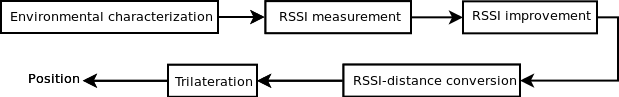
\includegraphics[width=0.7\textwidth]{process_hecops.png}
  \caption{Position calculation process}
\end{figure}

\subsubsection{Environmental characterization}
In order to calculate distance using the RSSI, we need to know a few environment variables. The strength of a received signal is described by the
following equation:
$$
P_r(d)= \frac{P_r(d_0)}{(\frac{d}{d_0})^n}
$$
$P_r(d)$ is the strength of the received signal at the distance $d$; \\
$P_r(d_0)$ is the strength of the received signal at the distance $d_0$; \\
$n$ is the path loss exponent;\\ \\
$P_r(d_0)$ and $d_0$ can be found by setting a value to $d_0$ (to 1 meter by convention) and measuring the value of the RSSI. 
We can then solve the equation for the path loss exponent, knowing the $P_r(d)$ and $d$:
$$ n = \frac{P_r(d_0) - P_r(d)}{10log_{10}(\frac{d}{d_0})} $$

\subsubsection{RSSI measurement}
The measurement of the RSSI has been implemented in EPOS. You can access the value of the strength of the last received signal through a radio
component. This value is also accessible through a node equipped with RSSI (cf. class diagram in appendix).

\subsubsection{RSSI improvement}
One way to improve the accuracy of the RSSI is to use heuristics. In the case of HECOPS, we measure the distance between two anchors and compare
it to the distance found by the conversion RSSI/distance. Then, we can adjust the value of the calulated position, knowing the deviation of the 
node.\\
A statistic estimator can also be set in order to predict and improve the values of the RSSI in order to counter the fluctuating values
of the RSS over time [12].

\subsubsection{RSSI distance conversion}
Once that we have the environmental parameters and that the RSSI value is as reliable as it can be, the value of the RSSI can be converted into
a distance value, using the previous equation solved for $d$. 
$$
d = d_0 \exp(\frac{P_r(d_0) - P_r(d)}{10n})
$$


\subsubsection{Trilateration}
Trilateration is a process that allows the calculation of the coordinates of a point, knowing three reference points and the distance between them
and the node of which we want the coordinates. The result of the process is the intersection of the three circles.\\
\begin{figure}[H]
  \centering
 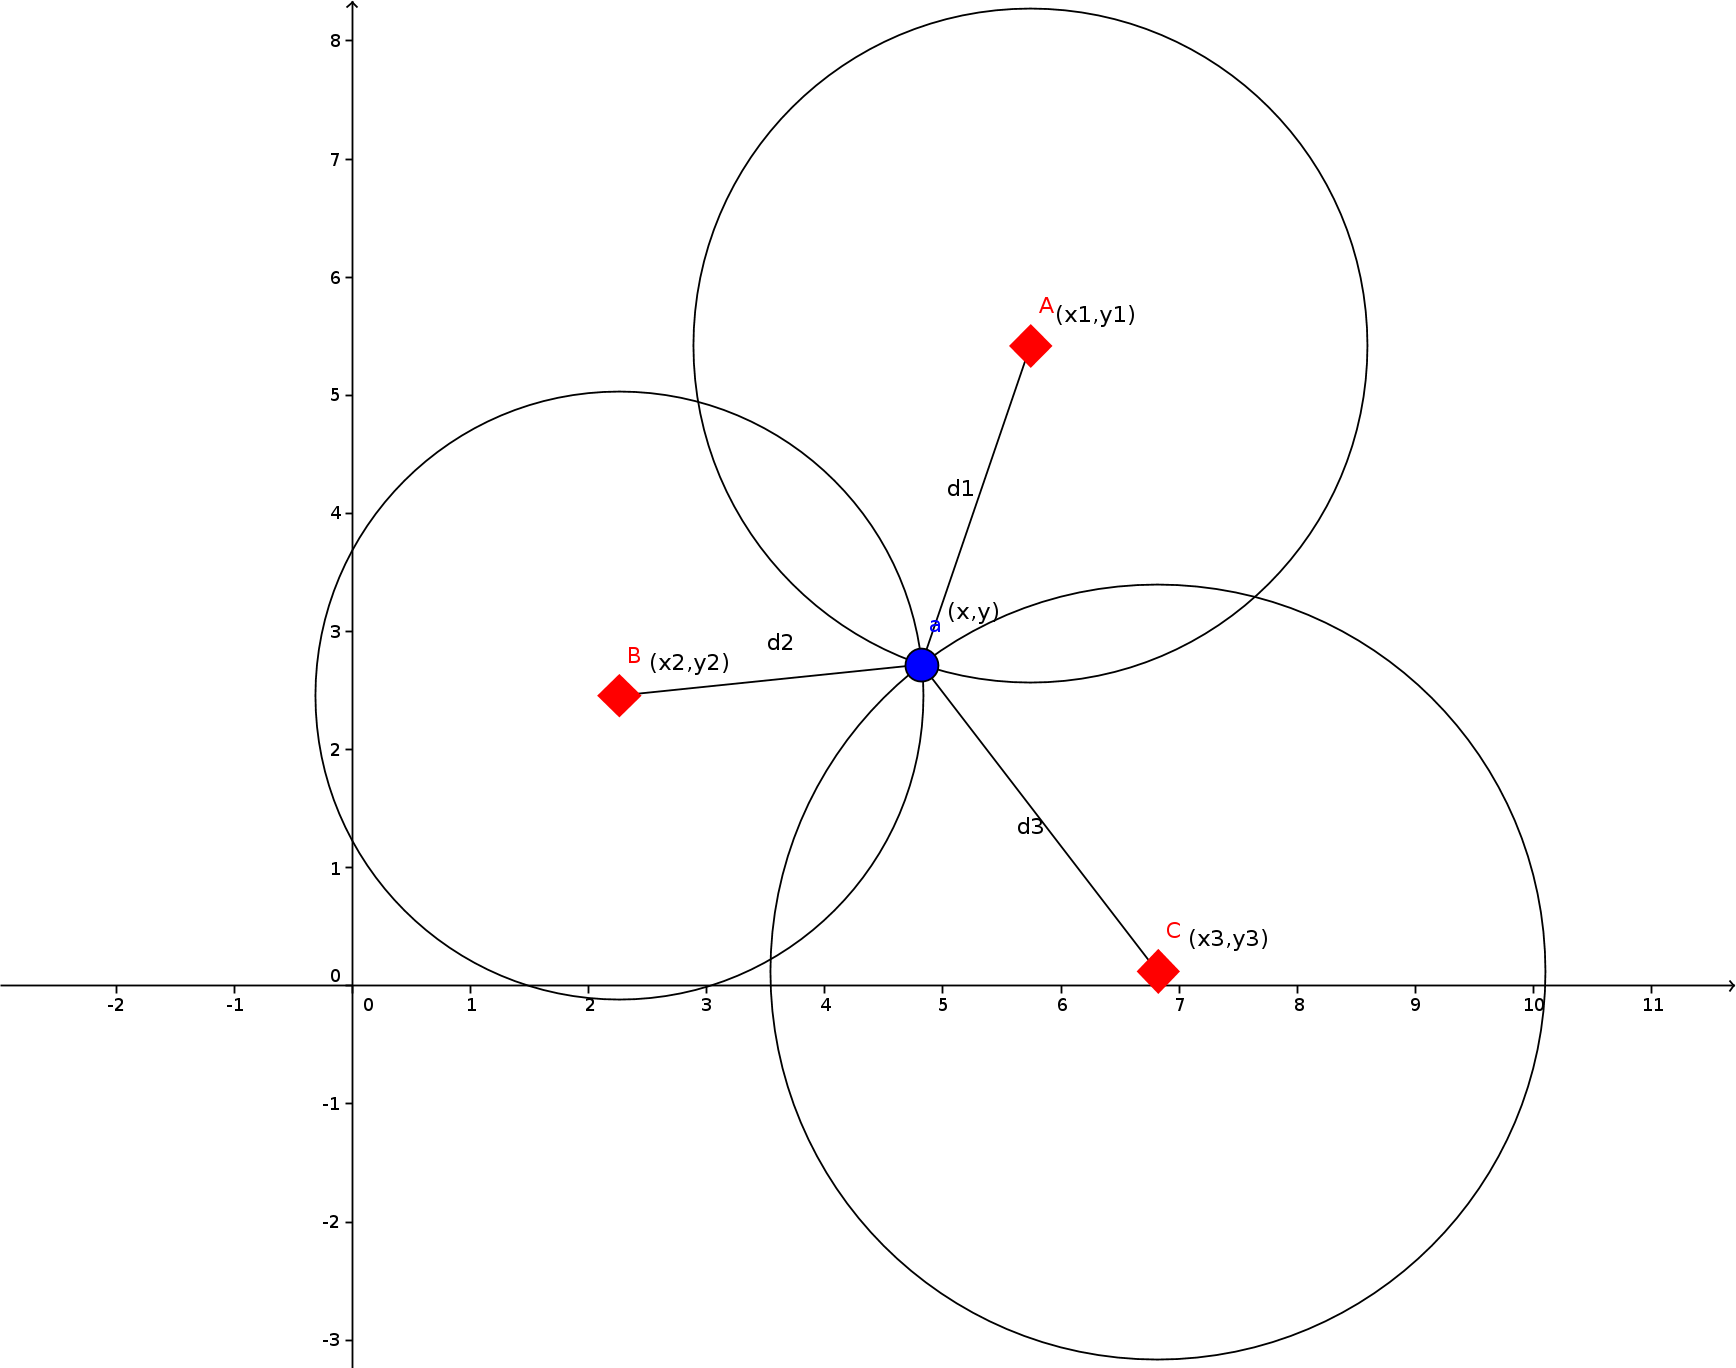
\includegraphics[scale=0.7]{trilateration.png}
  \caption{Trilateration process}
\end{figure}
\noindent
If we take the square of the euclidean distance between the references and the unknown node, we have a relation between the distances, the 
coordinates of the references and the coordinates of the unknown node: 
$$
\left\{
    \begin{array}{l}
     d_1^2 = (x_1 - x)^2 - (y_1 - y)^2 \\
     d_2^2 = (x_2 - x)^2 - (y_2 - y)^2 \\
     d_3^2 = (x_3 - x)^2 - (y_3 - y)^2 \\
    \end{array}
\right.
$$
We can solve these equations for x and y as follows:
$$
\left\{
    \begin{array}{l}
     x = \frac{AY_{32} + BY_{13} + CY_{21}}{2(x_1Y_{32} + x_2Y_{13} + x_3Y_{21})}\\
     y = \frac{AX_{32} + BX_{13} + CX_{21}}{2(y_1X_{32} + y_2X_{13} + y_3X_{21})}
    \end{array}
\right.
\begin{array}{l}
  A = x_1^2 + y_1^2 - d_1^2 \\
  B = x_2^2 + y_2^2 - d_2^2 \\
  C = x_3^2 + y_3^2 - d_3^2 \\
  X_{ij} = x_i - x_j \\ 
  Y_{ij} = y_i - y_j \\
\end{array}
$$
This value is however only as reliable as the reliability of the RSSI and of the accuracy of the math functions used. Indeed, there are several
things that can alterate the result: the RSSI instability (environment, bad sensors, ...), no RSSI improvement step and calculation approximation.
One way to improve the result is to use more than 3 references through multilateration to alterate the unknown variables. However, considering the
high computation effort necessary for this algorithm, it won't be taken into account in this paper. Many references on how to implement such
an algorithm can be found. If the calculation unit on the hardware allows it, it is interesting to implement such an algorithm to allow nodes that 
don't have direct access to a reference node to determinate their position. Of course, only nodes with a high confidence in their position should
be used to calculate another node's position, accordingly to the policy of HECOPS. Also, using a filter on the received strength signal can help 
to improve its reliability [12].

\subsection{eHECOPS}
A slightly different approach [11] has been done. In this process, we want to enhance the quality of the position through a better range measurement and more
sources of information.
The blue boxes represent what had been added or modified in the process of HECOPS:\\
\begin{figure}[H]
  \centering
 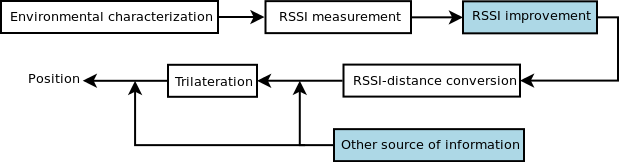
\includegraphics[width=0.7\textwidth]{process.png}
  \caption{Position calculation with eHECOPS process}
\end{figure}
\subsubsection{Ultrasonic sound sensors}
Ultrasonic sound sensors allow an accurate a reliable distance measurement. It can be used in two ways: to measure distance a calibrate position with 
this result, or as a source of information for an acoustic source localization.\\
The so far implemented version of ultrasonic sensors doesn't have enough functionalities to allow the second possibility. That is why the other strategy has 
been adopted.\\
Once again, the anchors and the mobile nodes won't have the same behavior, as the confidence in their position is not the same.
\begin{algorithm}[H]
\caption{Behavior of an anchor equipped with an ultrasonic sound sensor}
\begin{algorithmic}[H]
\IF{I receive coordinates from another node}
\IF{this node is mobile AND this node is in my range}
\IF{I can calculate the distance between us}
\STATE I send this measured distance to the mobile node so it can calibrate its position
\ELSE
\STATE this means that the estimation of its position is quite wrong, so I signal it
\ENDIF
\ENDIF
\ENDIF
\end{algorithmic}
\end{algorithm}
\begin{algorithm}[H]
\caption{Behavior of a mobile node equipped with an ultrasonic sound sensor}
\begin{algorithmic}[H]
\IF{I received information concerning the distance between an anchor and me}
\STATE calibrate my position if possible and necessary
\ELSE
\IF{I received information from an anchor node in my range}
\STATE measure the distance between us and calibrate my position
\ENDIF
\ENDIF
\end{algorithmic}
\end{algorithm}
\noindent
This improves significally the accuracy of the position, because the position calculation is based on the distance between reference nodes and 
mobile nodes.
\\
The following scheme shows the configuration in which a node will have its position calibrated.
\begin{figure}[H]
  \centering
 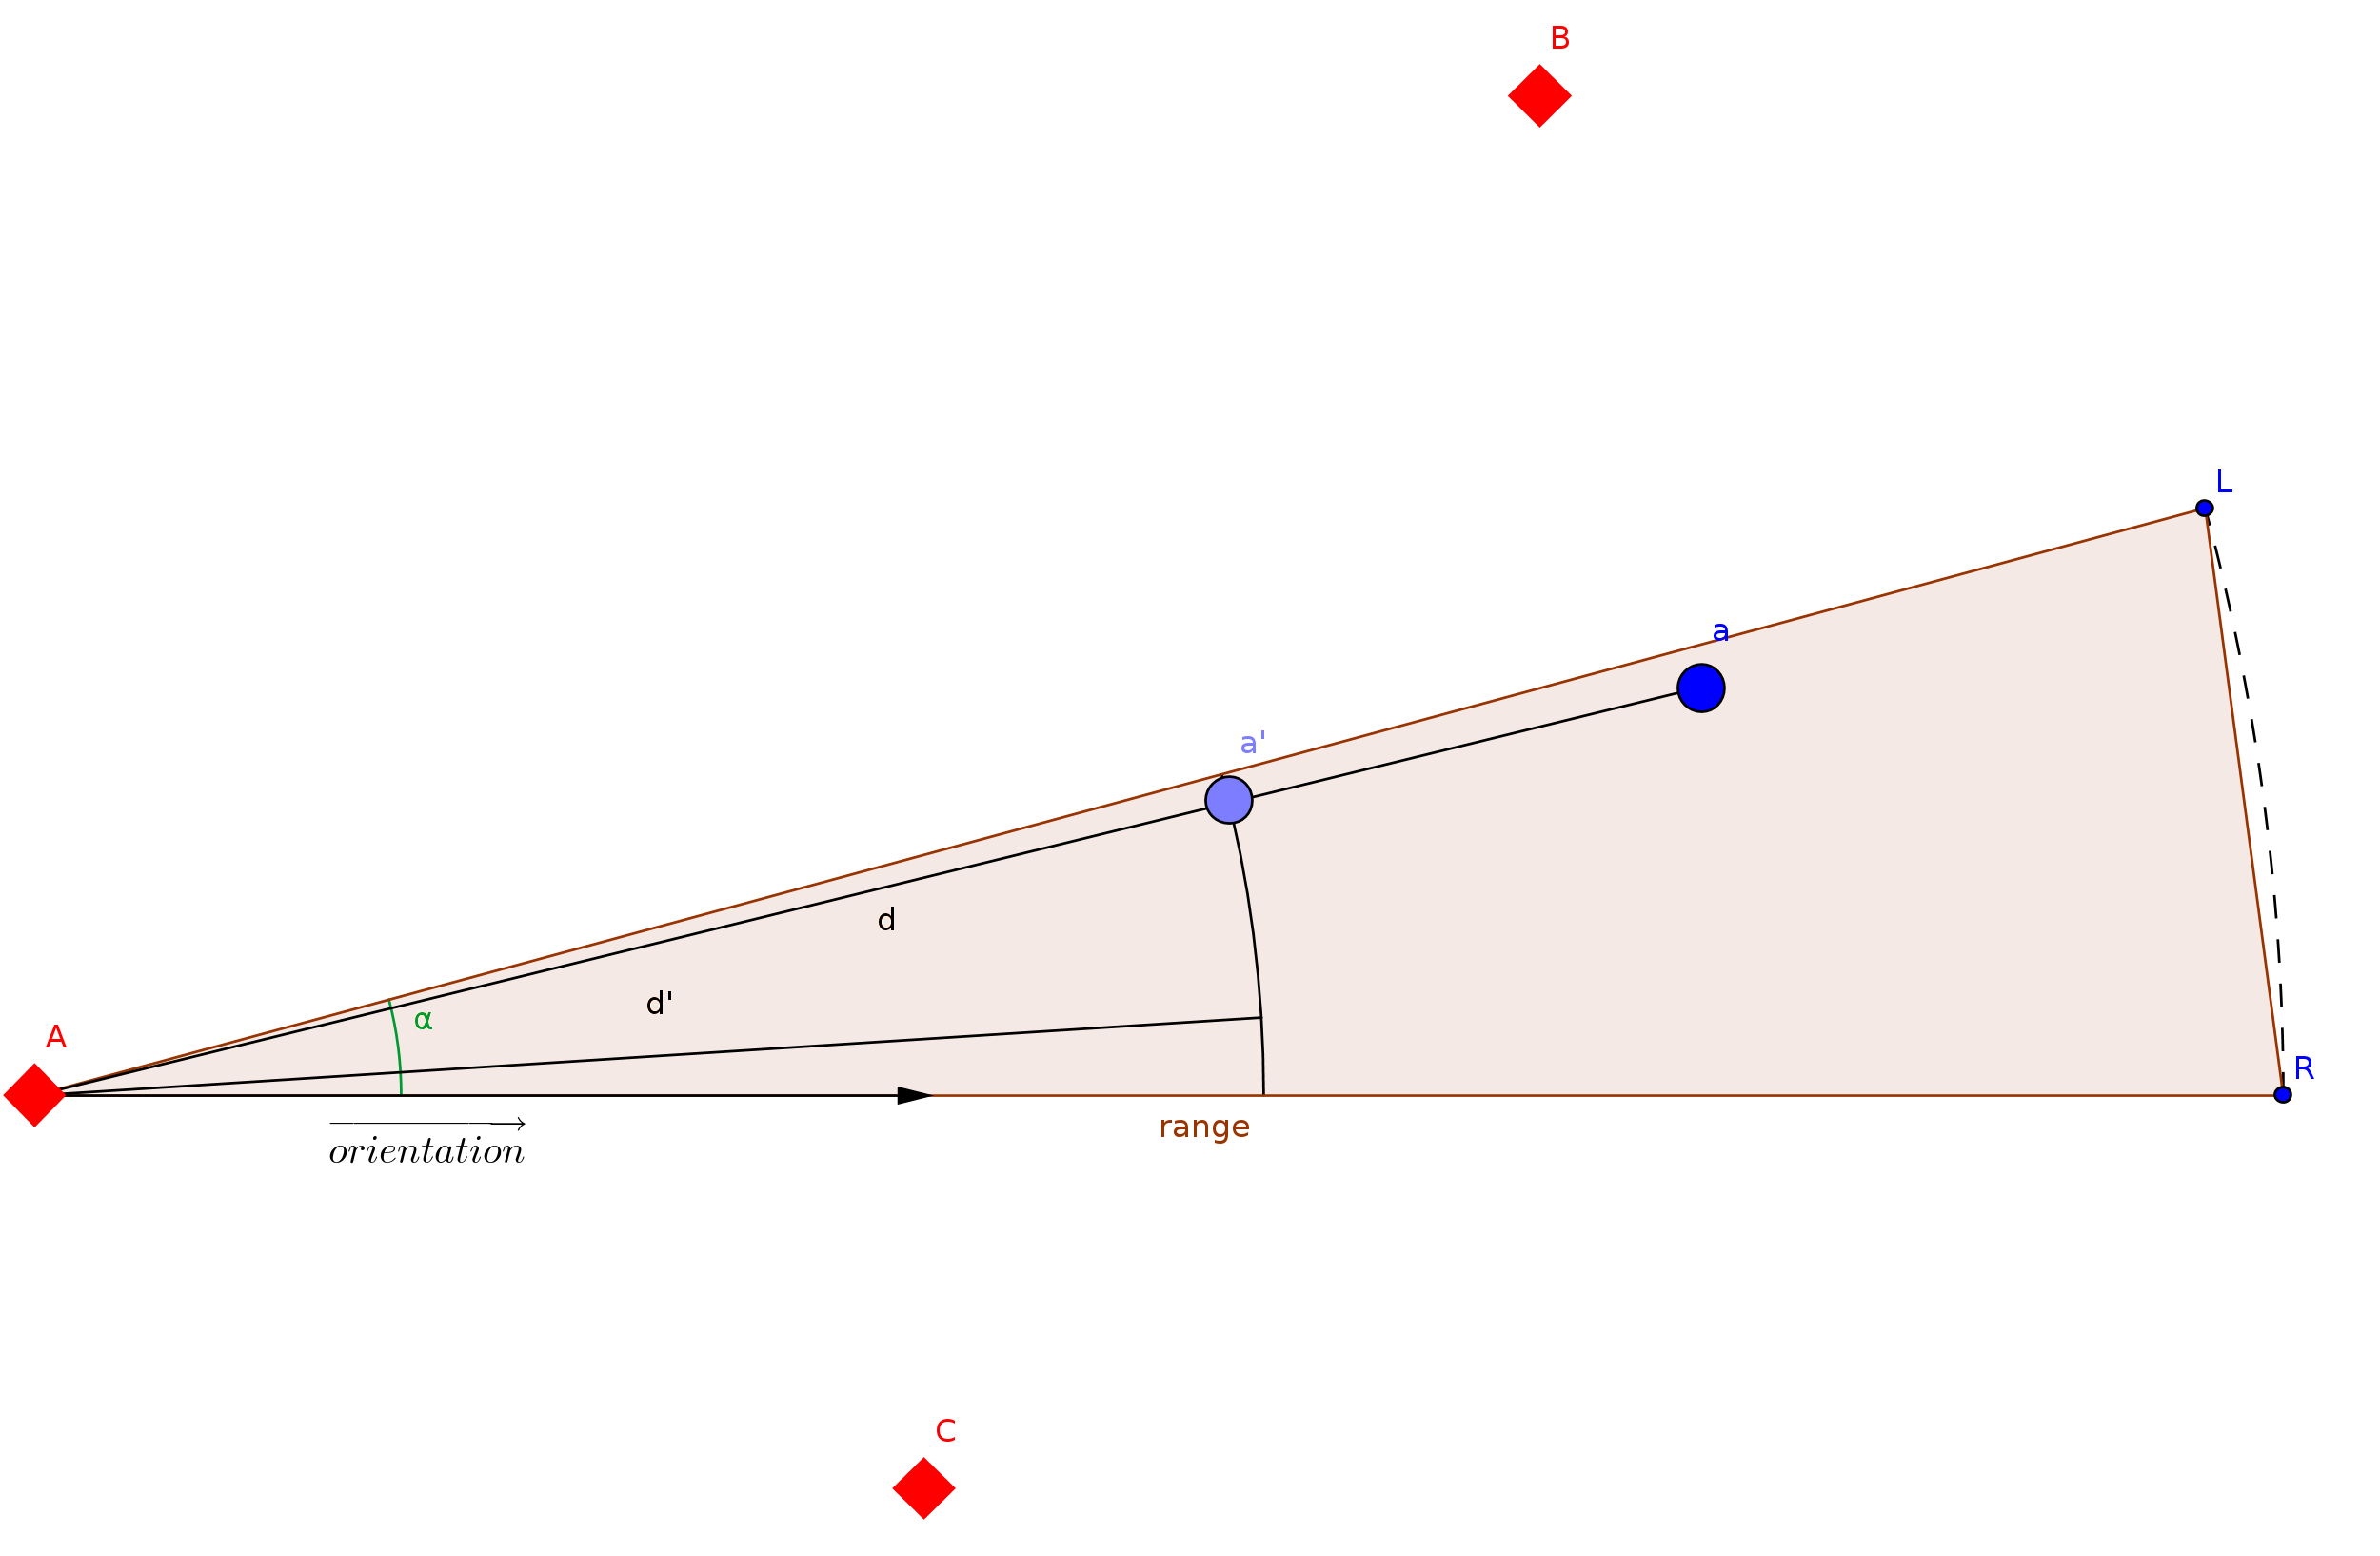
\includegraphics[width=0.7\textwidth]{triangle_us2.png}
  \caption{Calibration of the position of a node}
\end{figure}
In order to do this, a node equipped with ultrasonic sound sensors will have new information:\\
\begin{itemize}
  \item range min
  \item range max
  \item orientation // as a vector corresponding to the right side of the range triangle
  \item alpha // the angle of measurement
  \item R and L // the points forming the range triangle
\end{itemize}
The user only knows the information found on the datasheet. The triangle used in the algorithm remains to be built. Here is how it has been done in eHECOPS : 
To get R, we normalize the orientation vector so its norm equals the range. Then we can find the coordinates of R. Once we have R, we apply a 
rotation of alpha to the new orientation vector to find the coordinates of L.
$$
\left\{
    \begin{array}{l}
        x' = x\cos\phi - y\sin\phi \\
        y' = x\sin\phi + y\cos\phi
    \end{array}
\right.
$$
Then, once we have all this information, we can know if a node of coordinates (x,y) is inside the triangle by calculating the areas of the 
three triangles formed by the point, R, L and the node, and checking if it equals the area of the first triangle.\\
\begin{figure}[H]
\centering
\begin{subfigure}{.5\textwidth}
  \centering
  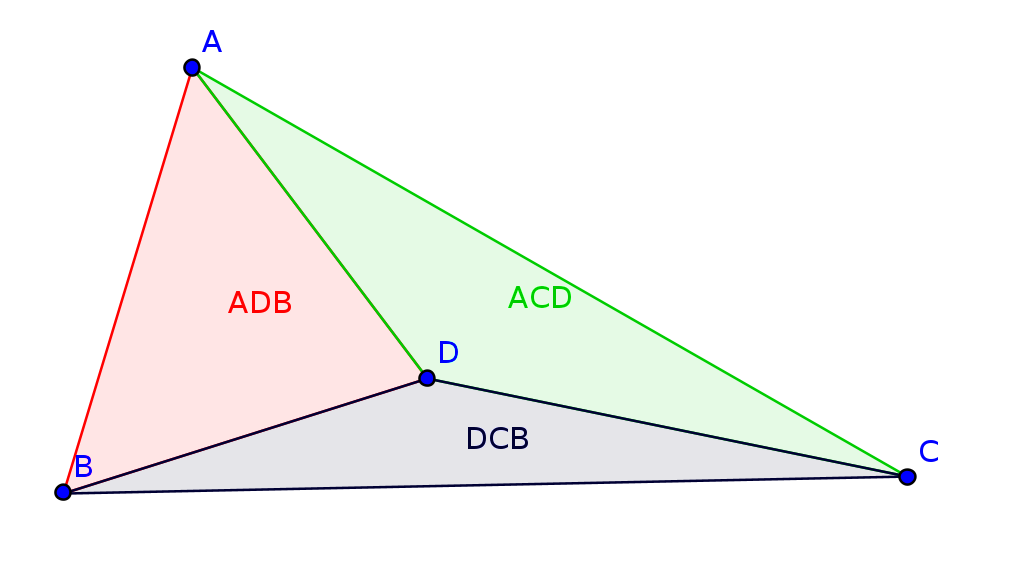
\includegraphics[width=.6\linewidth]{point_inside.png}
  \caption{ABC = ADB+ACD+DCB}
  \label{fig:sub1}
\end{subfigure}%
\begin{subfigure}{.5\textwidth}
  \centering
  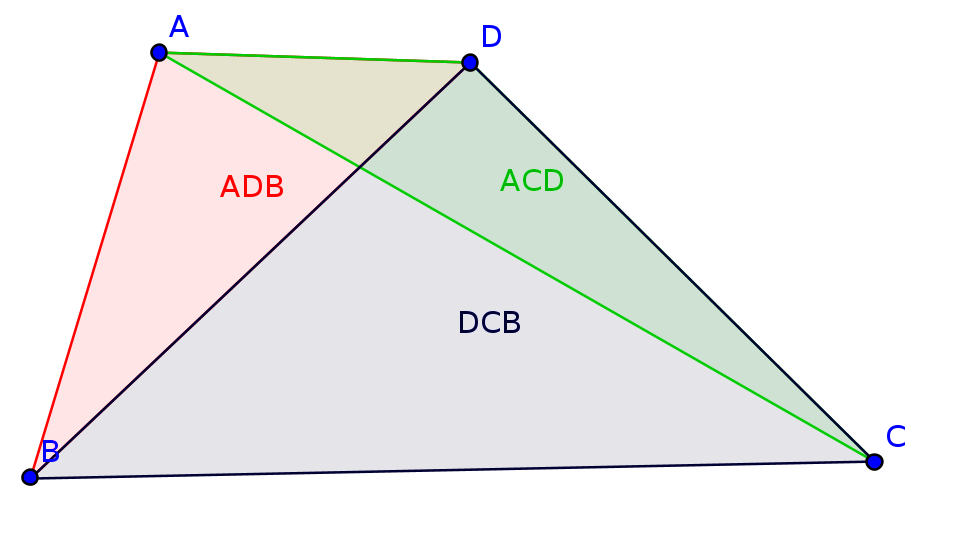
\includegraphics[width=.6\linewidth]{point_outside.png}
  \caption{ABC $\neq$ ADB+ACD+DCB}
  \label{fig:sub2}
\end{subfigure}
\caption{Possible configurations of 4 nodes}
\label{fig:test}
\end{figure}
\noindent
When a node receives the distance between it and an anchor, it has to calibrate its position in order to get the estimation closer to its true 
position. I therefore want the new coordinates to be in the range of the ultrasonic sensor, as close as possible to the measured distance and 
with the smallest distance to the original position. That is to say: we want the new position to be the projection of the coordinates on the range 
arc of circle of radius distance-measured-by-the-anchor and of center anchor. The way to do this is very simple:
$$\left(\begin{array}{l}
		      x_a' \\
		      y_a'
                    \end{array}\right)
=\frac{d}{d'}\left(\begin{array}{l}
		      x_{\overrightarrow{Aa'}} + x_a' \\
		      y_{\overrightarrow{Aa'}} + y_a'
                    \end{array}\right)
                    =\frac{d}{d'}\left(\begin{array}{l}	
		      x_a \\
		      y_a
                    \end{array}\right)
$$

\subsubsection{Near Field Communication}
The NFC technology allows two NFC sensors to communicate in a very short range. They can therefore exchange information when they are very close
from each other. One way to use this functionnality is to allow a node to communicate his position with a high level of confidence when communicating
with a node of high level of confidence. By doing this, we would insert another type of node in the localization algorithm: temporary anchor
nodes.
\begin{algorithm}[H]
\caption{Interruption handler when receiving a message from an anchor equipped with NFC}
\begin{algorithmic}[H]
\WHILE{I receive message from the anchor through NFC}
\STATE increase the confidence in my position and act like an anchor node
\ENDWHILE
\end{algorithmic}
\end{algorithm}
\noindent
Another way to use this functionnality is to exchange information between the nodes so they can combine
everything they know in order to have a more accurate estimation of their position.

\section{Results}
\subsection{RSSI}	
\subsubsection{Influence of the distance}
The expected experiments couldn't be performed due to bad weather condition. However, it would be interesting to get an experimental graph of
the value of the RSSI in function of the distance (with the scattering). This graph could help to determine how to improve the reliability of
the signal and check if the function is the same as the one determined during the characterization process.
\subsubsection{Influence of the angle}
During my tests, it has been noticed that the RSSI was highly depending on the angle between the transceiver and the receiver. That is why an
experiment in order to determine the influence of the angle on the value of the RSSI has been set up. Two types of antenna are available with the
EPOSMote: internal or external. The point of this experiment was to compare these antennas. 
Two motes were put 1.5m away from each other. The receiver was put on a protractor. The graphes below represent the results for 10
measurements at a fixed angle.\\
A first way to present the result is to look at the variation of RSSI in function of the angle.
\begin{figure}[H]
  \centering
 \includegraphics[width=0.7\textwidth]{rssi_antenna.jpg}
  \caption{Variation of RSSI}
\end{figure}
\noindent
Another way is to look at the standard deviation for each antenna at different angles. This gives an idea of the stability of the value of RSSI.
\begin{figure}[H]
  \centering
 \includegraphics[width=0.7\textwidth]{sdev_antenna.jpg}
  \caption{Standard deviation}
\end{figure}
\noindent
Unexpectedly, the external antenna did not show better results than the internal antenna. The signal is stronger but varies just as much as the
signal received by the internal antenna.

\subsection{Distance measurement}
An experiment has been done in order to validate the measurement of distance using the value of the RSS. For each step of this experiment, two
nodes were put d cm away from each other. Then the distance was calculated based on the value of the RSS for 10 samples. The following graph
represents the repartition of these calculations and the average error during this test. The orientation between the nodes has been kept
as constant as possible but some changes of condition due to moving the nodes from place to place may have been inserted.
\begin{figure}[H]
\centering
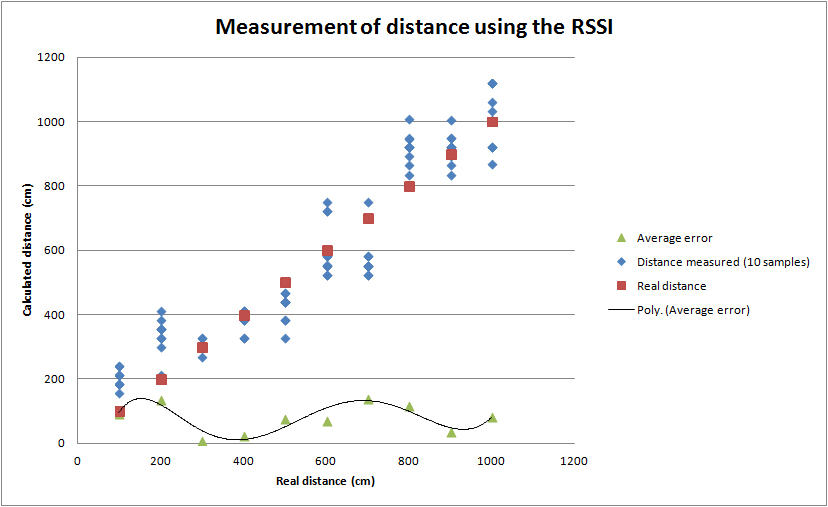
\includegraphics[width=0.7\textwidth]{distance_measurement.jpg}
\caption{Measurement of distance using the RSSI}
\end{figure}
\noindent
It may be interesting to realize the same type of experiment with the signal improvements.
\subsection{Localization algorithm}
The localization algorithm was tested in two situations with the same configuration but a different environment. A mobile node followed a defined
path and tried to localize its position when reaching a point of reference.\\
For the first test (blue), reference nodes were placed on an obstructed area with a lot of potential interferences: a closed room with tables, panels 
obstructing the signals and computers, wifi network and lamps creating potential interferences. \\
For the second test (green), reference nodes were placed on a clear outside area.
\begin{figure}[H]
\centering
 \includegraphics[width=\textwidth]{way_inside_outside.png}
\caption{Estimation of position inside and outside a building}
\end{figure}
\noindent
As expected, the second experiment presented results closer to the reality. One thing that is important to note is that during these experiments,
the nodes have been manually rotated in order to get an average value of RSSI as reliable as possible. This has been done in order to avoid the 
problem of the dependency of RSSI on the orientation of the circuit. This problem is more common when using integrated antenas (which have been
used during this test). Therefore, the mobile  node had to get as many values of RSSI in order to estimate the distance btween
it and the node. These values were not very reliable and even one (among three) wrong estimation of the distance can lead to a very wrong result. \\
The following scheme presents the problem. Considering quite good distance estimations between the mobile node and the anchor nodes B and C (less than 
5\% of error)and several distance estimations, the node calculates its position. The percentage under the estimations represents the error percentage 
of  the estimation of the distance between the anchor node A and the mobil e nod e. s shown previously, an error of a 100\% in the estimation of the                 
 distance  is quite likely for small distances. Therefore, such an error of estimation is likely too.                                          
                            
\begin{figure}[H]
\centering
\begin{subfigure}{.5\textwidth}
  \centering
  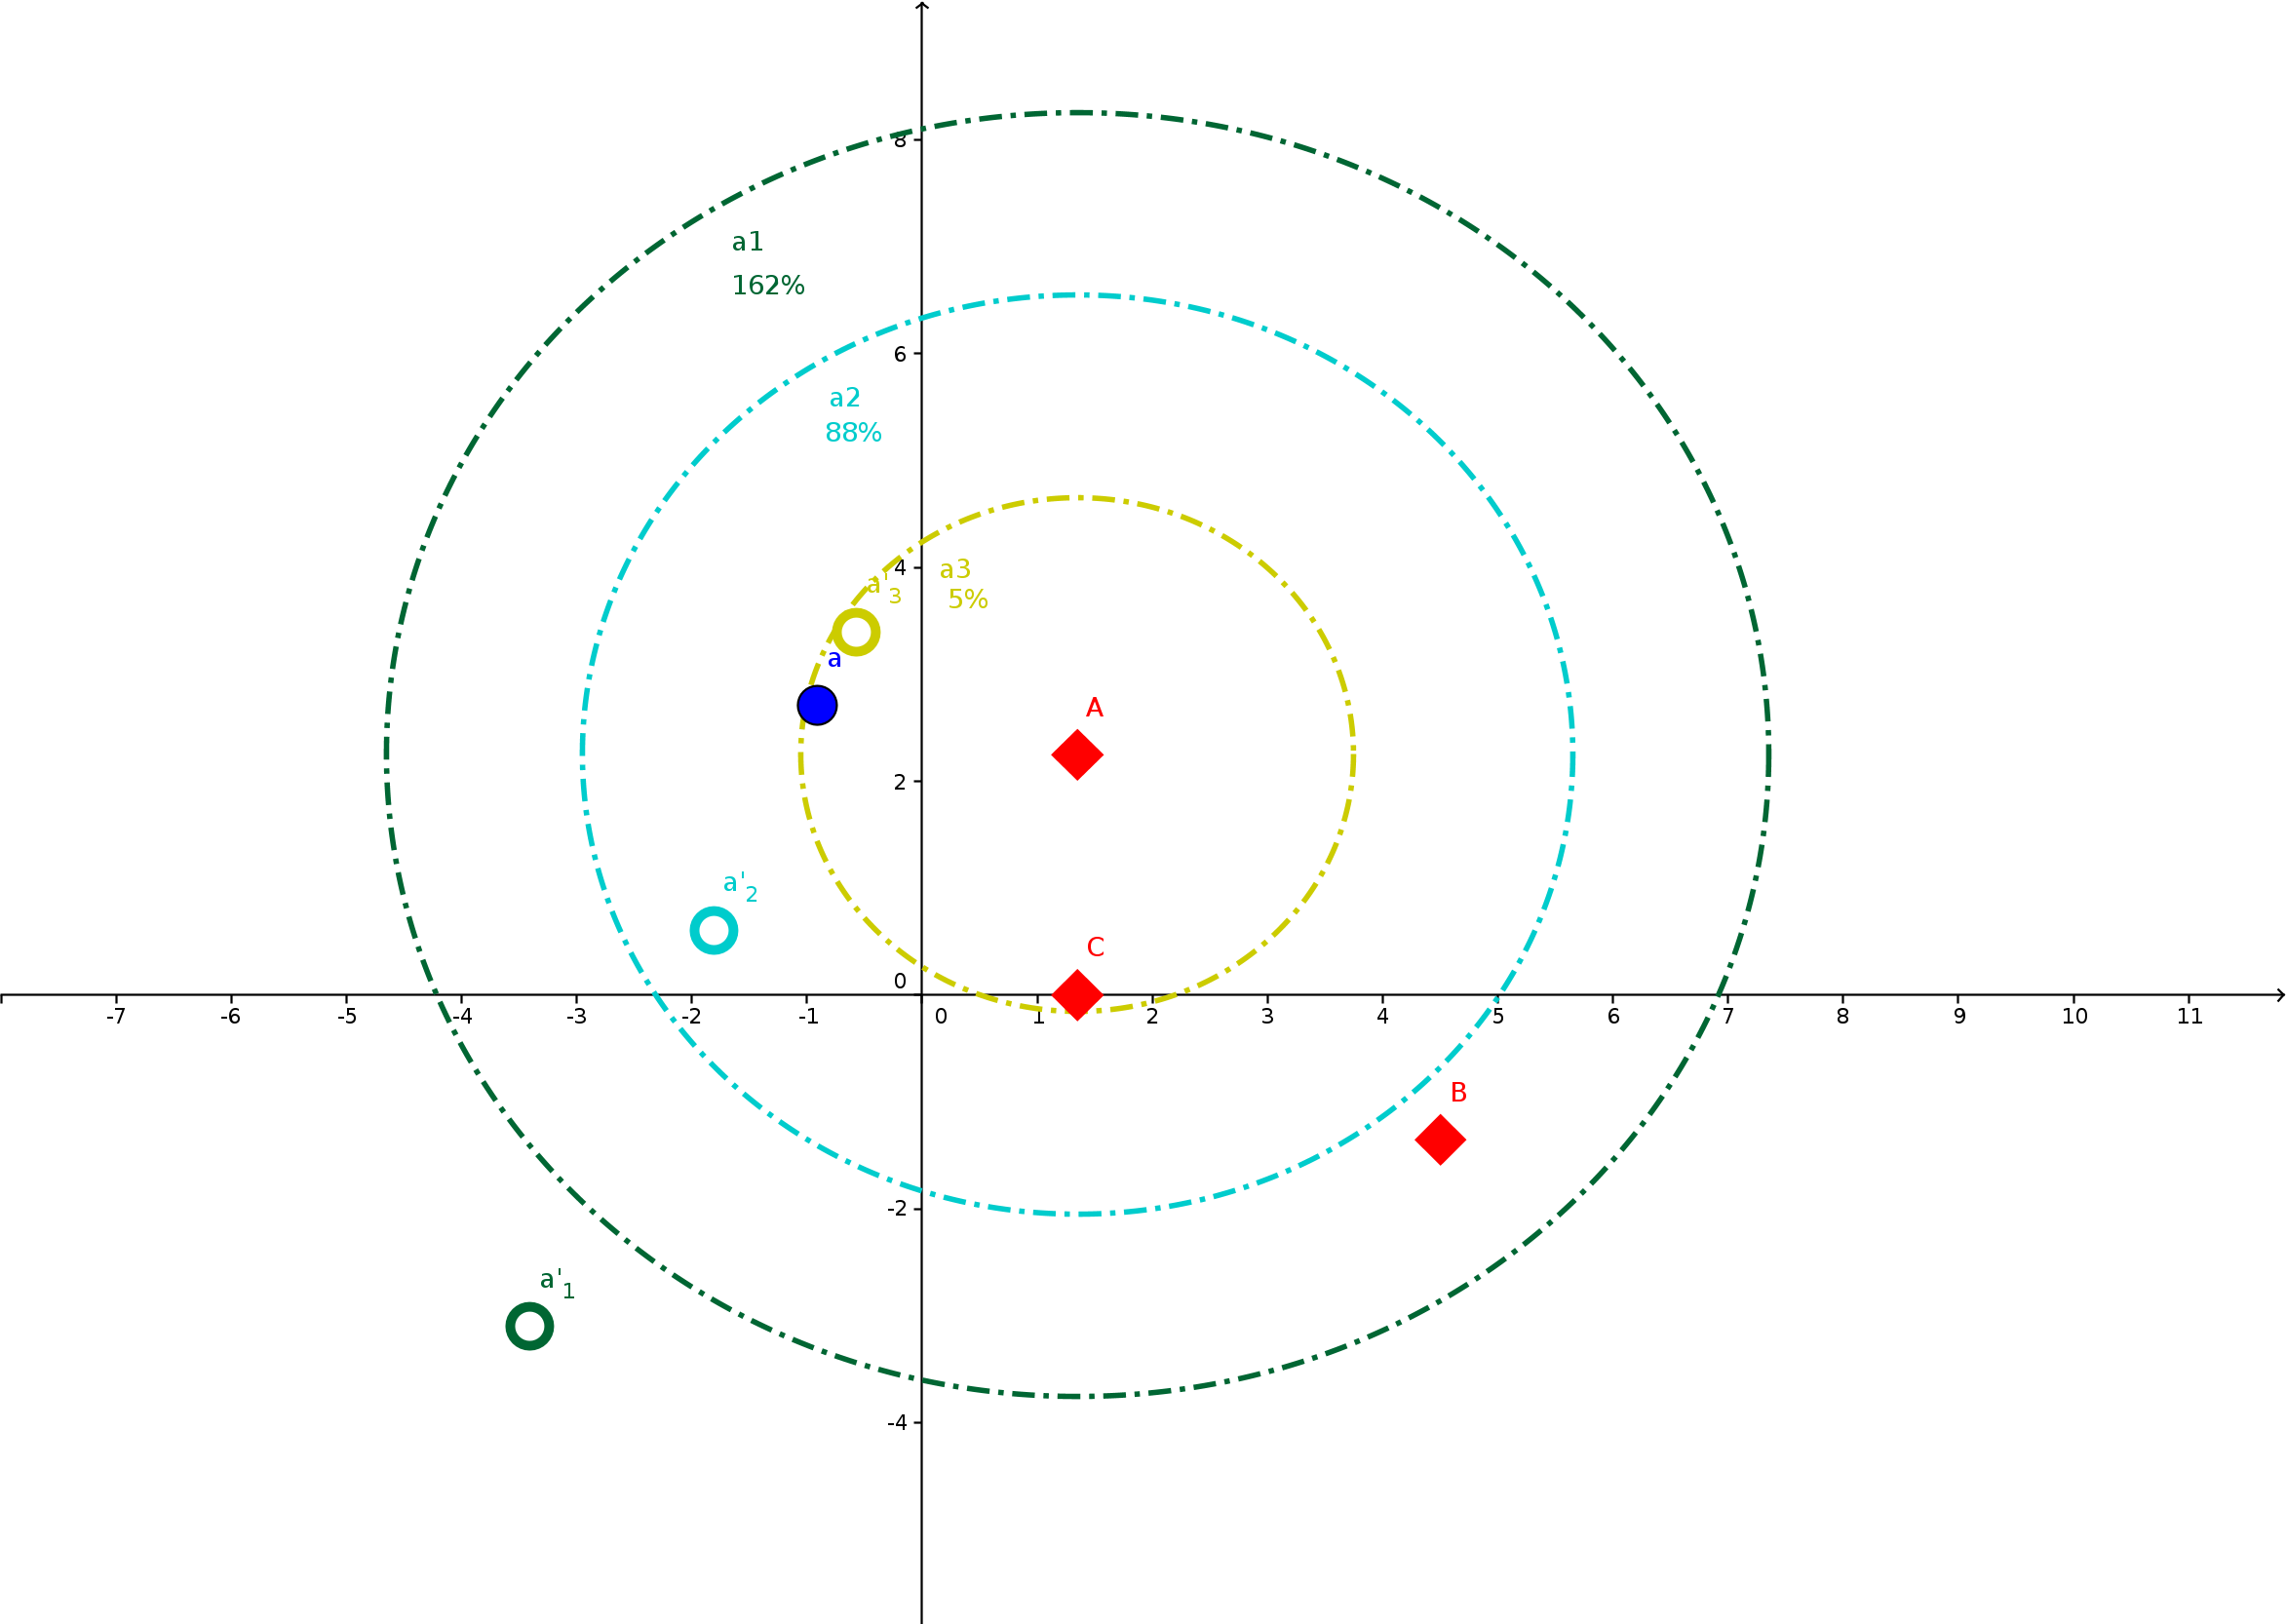
\includegraphics[width=\linewidth]{trilateration_error.png}
  \caption{Estimated positions with different errors}
  \label{fig:sub3}
\end{subfigure}%
\begin{subfigure}{.5\textwidth}
  \centering
  \includegraphics[width=0.8\linewidth]{distance_error.jpg}
  \caption{Error of position estimation with different errors of estimation of distance}
  \label{fig:sub4}
\end{subfigure}
\caption{Position estimation error with the trilateration method }
\label{fig:trilateration_errors}
\end{figure}
\noindent
This problem of uncertainty considering the RSSI remains to be addressed. The use of multiple source seeks to improve the reliability of the
range measurement. Here it is another problem concerning the RSSI itself.\\
Filters should be a good solution to get better values of RSSI. An interesting approach is to add a plausibility filter [13]. Basically, this
paper presents a plausibility filter that only allows the values that lead to a movement that does not exceed a certain speed. The resulting
filter is presented hereinunder.
$$
\Delta d_{max} = (t_n - t{n-1})v_{max} 
$$

$$
d'_n = \left\{ \begin{array}{ll}
                d'_{n-1} + \Delta d_{max,n} & if (d_n - d'_{n-1}) > \Delta d_{max,n} \\
                d'_{n-1} - \Delta d_{max,n} & if (d'_{n-1} - d_n) > \Delta d_{max,n} \\
                d_n & else 
               \end{array}
\right.
$$
Another interesting filter would be a Kalman filter. In this filter, a time discrete state space observation by means of a state and an
observation equation is used in order to model the motion of a moving node. With this filter, we can try to predict the position of a mobile
node. Another interesting of this feature is the fact that it uses a state variable. We can therefore include other sources of information and
try to predict their values too. This could be an interesting feature for the enhanced HECOPS that uses multiple sources.\\
\begin{figure}[H]
\centering
 \includegraphics[width=\textwidth]{Basic_concept_of_Kalman_filtering.png}
\caption{Basic concept of Kalman filtering (source: wikipedia.org)}
\end{figure}
\noindent
However, these filters may take too much computation effort for an embedded system. We can therefore think of ways to lessen the amount of
computation time. An interesting idea would be to take "advantage" of the fact the the signal is intrinsically unstable. Therefore we can
approximate the conversion RSSI-distance and avoid some mathematical calculations (such as an exponential).
\begin{figure}[H]
\centering
 \includegraphics[width=0.7\textwidth]{wout_app.jpg}
\caption{RSSI function of distance}
\end{figure}
\begin{figure}[H]
\centering
 \includegraphics[width=0.7\textwidth]{with_app.jpg}
\caption{RSSI function of distance approximated}
\end{figure}

\subsection{Ultrasonic sound sensor and NFC}
The necessary features to fully test these features haven't been implemented yet. A basic test simulating entries from the ultrasonic sound
sensor have been implemented on a node trying to improve the accuracy of its position. In this test, we assume that the said node has a knowledge
of its position accurate enough to be considered inside the range triangle of a reference node. In these conditions, the mobile node is able to
improve the accuracy of its position as much as the accuracy of the ultrasonic sound sensor allows it.
\begin{figure}[H]
\begin{center}
 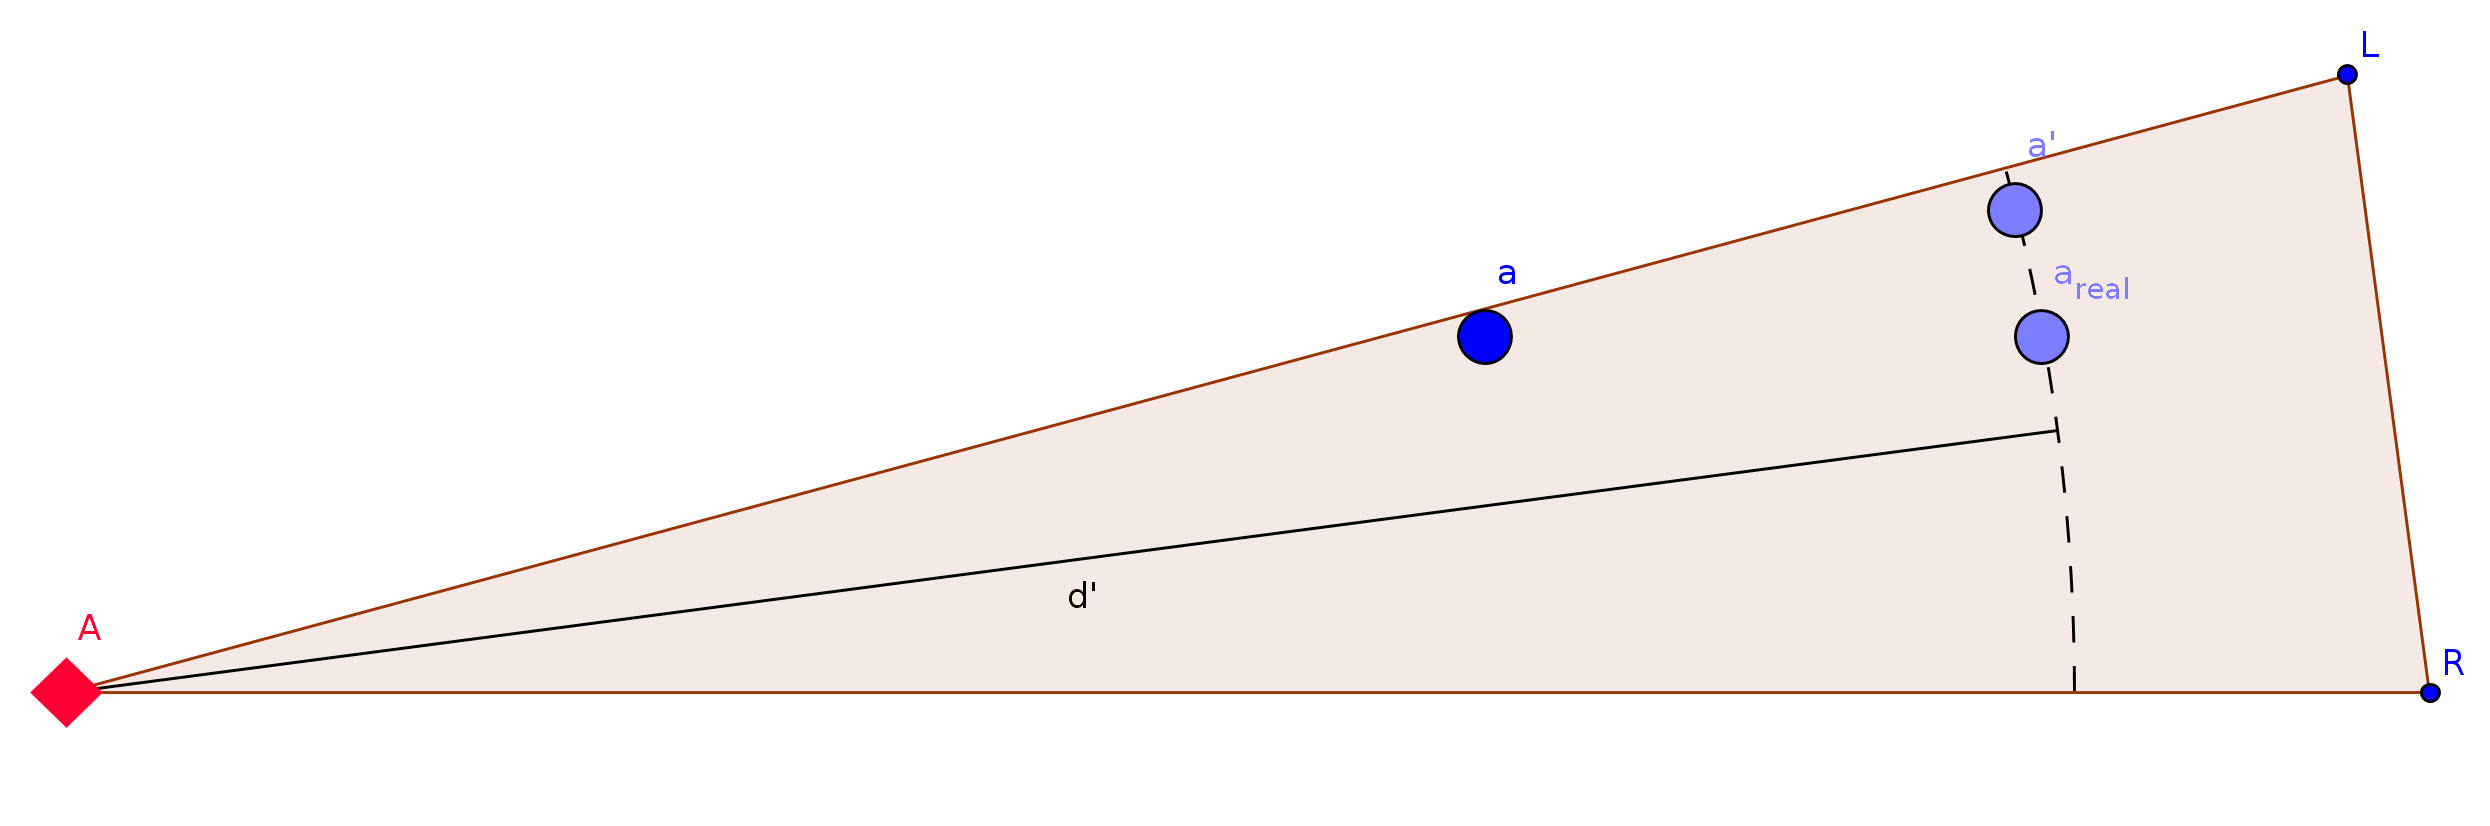
\includegraphics[width=0.7\textwidth]{triangle_us.png}
 % hecops_results.png: 1818x1433 pixel, 300dpi, 15.39x12.13 cm, bb=0 0 436 344
\end{center}
\caption{Improvement of position estimation with ultrasonic sound sensor entries}
\end{figure}
\noindent
On this scheme, we can see the range triangle of the ultrasonic sound sensor of the anchor node A, the estimated position of B, the arc of circle
of position possibilities based on the measurement of distance and the choice of the new position of B.

\section{Conclusion and future work}
Our algorithm, though functional, is very dependant on the quality of the range measurements. The quality of the position estimation is quite good
when all the range measurements it depends on are good. The efforts put into improving these range measurements can therefore highly improve the
quality of the localization. There are ways to improve the value of the RSSI, but this method of range measurement has its physical limitations.
Including other sources of information appears as a feasible way to improve the range measurements. If a few nodes in the network provide this
type of information, it will improve the quality of the knowledge of the positions of the nodes of the whole network. \\
Therefore, it would be interesting to research on ways to improve the range measurements (signal improvement, multiple sources) and to start
thinking of applications for this feature.
\subsection{Personnal feedback}
Working at LISHA has been a great experience. I have really enjoyed working in this environment, and the subject was very interesting. \\
However, I deeply believe that I could have done much more if I had had more resources. By resources, I mean two things. The first was one space.
It was hard to set up experiments because I did not have enough room to run my tests. Inside was a very closed space with a lot of interference
and a lot of people to bother. Outside, I had to go to the other side of the campus and build a homemade cartesian coordinates system. Then the
measurements were hard to make accurately because of this homemade system. Moreover, my experiments depended on the weather: when it was raining
or had rained, I coudn't bring electronic devices there, and when it was too sunny, I couldn't let my computer out under the sun for too long.
The second resource I missed was the hardware that I was supposed to use. It may be a better idea to start a project relying on other projects
when these projects are done and validated. This way, I could have focused on some other things instead of waiting for them. I am not saying that
it is bad that these projects were not done, but that it would have been more comfortable if I didn't wait for them. This lack of resources
sometimes lead me to situations when I didn't know what to do and got demotivated. Having a flexible workplan was a great thing to work on what I
wanted to, but contributed to the feeling of not knowing what to do.\\
That being said, I really appreciated having a flexible workplan. I was not so motivated  by the original workplan, and am really glad
that I have been able to work on something that interested me more. I appreciated the fact that I never stayed stuck for a long time. Whenever I
had a problem or needed something, I could find someone at the lab who could help me with my problem, or give me what I needed. I have learned a
lot while working at LISHA and it definitely fills in my education: design a program for a new platform, familiarize myself with a new operating
system (use and maintain), set up experiments, get in touch with embedded system issues, find relevant related work, learn a new programming
language, work in a different environment, different language, different culture... I think that all these new skills will be helpful in both my
personnal and professional life.\\
I am proud to be the first (of many, I hope) French student who came to LISHA. I am really thankful to everyone who contributed to this
life experience.

\section{References}
[1]
Ricardo Reghelin and Antônio Augusto Frohlich -
Laboratory for Software and Hardware Integration - UFSC -  
A decentralized location system for sensor networks using cooperative calibration and heuristics -
\url{http://www.lisha.ufsc.br/pub/Reghelin_MSWIM_2006.pdf}\\
{[2]}
Mohammad Reza Gholami -
Communication Systems Group - Department of Signals and Systems chalmers university of technology - Gothenburg, Sweden 2011 -
Positionning algorithms for wireless sensor networks -
\url{publications.lib.chalmers.se/records/fulltext/138669.pdf} \\
{[3]}
Mingfei Wang, Linlin Ci, Ping Zhan, Yongjun Xu -
School of Computer Science and Technology, Beijing Institute of Technology, Beijing, 100081, China -
Beijing Institute of Information Technology, Beijing, 100085, China -
Laboratory of Wireless Sensor Networks, Institute of Computing Technology, Chinese Academy of Sciences, Beijing, 100080, China -
Accoustic source localization in wireless sensor networks - 
\url{http://ieeexplore.ieee.org/stamp/stamp.jsp?tp=&arnumber=4426998&tag=1}\\
{[4]}
Youngbin You and Hojung Cha - 
Department of Computer Science, Yonsei University - 
Seodaemum-gu, Shinchon-dong 134, Seoul 120-749, Korea -
Scalable and low cost acoustic source localization for wireless sensor networks - 
\url{citeseerx.ist.psu.edu/viewdoc/download?doi=10.1.1.105.4426&rep=rep1&type=pdf}\\
{[5]}
LIU Yong, HU Yu Hen, PAN Quan - College of Automation, Northwestern Polytechnical University, Xi’an 710072, P. R China -
University of Wisconsin, Madison, WI 53706, USA -
Energy-efficient robust acoustic source localization with local outlier rejection in wireless sensor networks -
\url{http://ieeexplore.ieee.org/stamp/stamp.jsp?tp=&arnumber=6000477}\\
{[6]}
Florian Michahelles, Frederic Thiesse, Albrecht Schmidt, and John R. Williams - 
Carnegie Mellon Universit - 
Pervasive RFID and Near Field Communication technology - 
\url{http://ieeexplore.ieee.org/stamp/stamp.jsp?tp=&arnumber=4287450}\\
{[7]}
B. Sc. Björn Bittins,Prof. Dr. Jürgen Sieck -
INKA research group, HTW Berlin, Wilhelminenhofstr. 75A, 12459 Berlin - 
Multimodal and collaborative localisation service for diverse environments - 
\url{http://ieeexplore.ieee.org/stamp/stamp.jsp?tp=&arnumber=6377625}\\
{[8]}
James L Crowley and Yves Demazeau - 
LIFIA (IMAG) - 
Principles and techniques for sensor data fusion - 
\url{http://www-prima.inrialpes.fr/jlc/papers/SigProc-Fusion.pdf}\\
{[9]}
University of Toulouse - 
Particular methods and data fusion\\
\url{http://www.math.univ-toulouse.fr/~baehr/meteo_SMAI_DSNA/Pres/Pres_Caron.pdf}\\
{[10]}
Ren C. Luo Fellow, IEEE Ogst Chen, *L.C. Tu-
Department of Electrical Engineering, Department of Opto-Mechatronic - 
National Chung Cheng University 160, Shang-Shing, Ming-Hsiung, Chia-Yi, Taiwan 621, R.O.C. 
Nodes localization through data fusion in sensor network - 
\url{http://ieeexplore.ieee.org/stamp/stamp.jsp?arnumber=01423514}\\
{[11]}
Chuan-Chin Pu, Chuan-Hsian Pu and Hoon-Jae Lee (2011). Indoor Location Tracking Using Received Signal
Strength Indicator, Emerging Communications for Wireless Sensor Networks, (Ed.), ISBN: 978-953-307-082-7,
InTech, Available from: \url{http://www.intechopen.com/books/emerging-communications-for-wireless-sensor-
networks/indoor-location-tracking-using-received-signal-strength-indicator} \\
{[12]}
Enhanced Location Algorithm with Received-Signal-Strength Using Fading Kalman Filter in Wireless Sensor Networks - 
Jieyang Yi, Liang Zhou - 
IEEE Conference Publishing - 
School of Communication and Information Engineering - 
University of Electronic Science and Technology of China, Chengdu SiChuan 611731, China - 
\url{http://ieeexplore.ieee.org/stamp/stamp.jsp?tp=&arnumber=6089930}\\
{[13]}
RSSI-based Indoor Localization using Antenna Diversity and Plausibility Filter -
Andreas Fink, Helmut Beikirch -
Institute of Electronic Appliances and Circuits -
Department of Computer Science and Electrical Engineering - 
University of Rostock -
\url{http://ieeexplore.ieee.org/stamp/stamp.jsp?tp=&arnumber=4907821}
\newpage 
\appendix
\appendixname
\\ \\Two guides have been written. One for users and one for developpers. To simplify the task of finding useful information, they have been written
in the format of a Frequently Asked Questions (FAQ).
\section{User guide}
\textbf{Q - What does this code do?} \\
\textbf{A - }The first question to ask yourself indeed. This project contains code that is to be uploaded on an EPOSMote. In particular, it 
contains the implementation of HECOPS, a self localization algorithm of a node in a wireless sensor network. Therefore, all the necessary structures
of nodes are also contained in this package. 
\\ \\
\textbf{Q - How do I use it?}\\
\textbf{A - }Before reading the answer to that question ,you should read the answer to \textquotedblleft Is there any initialization
step?\textquotedblright.
In order to use the localization algorithm for EPOS, the header files node.h and location\_algorithm.h should be included. \\
A node, as described in the header file node.h, can be decorated with several functionalities. Each node can apply a strategy to determinate 
their position. This strategy, described in location\_algorithm.h, has to be chosen by the user at the instanciation of the node.
Please refer to the constructors and to the following example to understand how instanciate such an object. \\
As the localization algorithm should be pervasive, it will run forever once it is launched. The coordinates of the node will be updated
as the algorithm runs. If you plan on using the coordinates of the node, make sure that you run the algorithm in a thread synchronized
with the execution of the algorithm on the other nodes.\\
Code example
\begin{figure}[H]
\begin{verbatim}
#include <node.h>
#include <location_algorithm.h>

__USING_SYS

NIC * nic;
Ultrasound* node;
EHECOPS* ehecops;
int maxRang=20; // meters
int minRange=5; // centimeters
int alpha=15; // measuring angle, degrees
Coordinates orientation(1,0); // orientation of the sensor

int main() {
    // allocation of the necessary structures
    ehecops = new EHECOPS();
    nic = new NIC();
    
    // create the node with all its functionalities
    node = new Ultrasound(new RSSI(new Anchor('A',0,0,ehecops, nic)),
                          maxRange,
                          minRange,
                          alpha,
                          &orientation);

    // apply the localization strategy
    node->location(node);
    
    delete node;
    return 0;
}
\end{verbatim}
\caption{Example of code for the creation and use of an anchor node equipped with RSSI and ultrasonic sound sensor}
\end{figure}
\noindent
\textbf{Q - Is there any initialization step?}\\
\textbf{A - }If you plan on using the RSSI, you should set up the environmental parameters first. The file characterization.cc will help you to do so.
In this file, you can measure these parameters step by step. The environmental parameters depend on the physical place where the nodes will be put.
\\ \\
\textbf{Q - How do I create a node?} \\
\textbf{A - }Please refer to the code example hereinabove.
\\ \\
\textbf{Q - What can I do with a node?} \\
\textbf{A - }The main purpose of this code is to run the localization algorithm. However, you can access to all the capabilities of a node that are
publicly declared in the header file.
\\ \\
\textbf{Q - Can I add functionalities to a node?} \\
\textbf{A - }In order to do that, you have to re-instanciate an object containing all the capabilities that you want the node to have. This is not
meant to be done dynamically.
\\ \\
\textbf{Q - What is a strategy?} \\
\textbf{A - }A strategy corresponds to the algorithm that you want to use to locate the node.
\\ \\
\textbf{Q - What strategies can I choose? How do I choose that strategy?} \\
\textbf{A - }You create a node with the strategy that you want it to use, so you instanciate an object strategy. Please refer to the code example 
hereinabove. At this point, the only fully functional strategy is HECOPS, and some work is being done on eHECOPS.
\\ \\
\textbf{Q - Who can I contact if I have more questions?} \\
\textbf{A - }Thibault Rihet: \href{mailto:thibault@lisha.ufsc.br}{thibault@lisha.ufsc.br}


\newpage
\section{Developper guide}
\textbf{Q - Where do I start?} \\
\textbf{A - }The first thing you should do is get familiar with the global architecture described in the class diagram hereinunder. Then, use the 
user guide section to familiarize yourself with the architecture.
\\ \\
\textbf{Q - What part of the code does what? How are the files organized} \\
\textbf{A - }The architecture is described in the class diagram hereinunder. The two main sections of the code are contained in the classes Node and 
Location\_Algorithm. \\
The class Node contains everything directly related to the structure of the node. All the nodes have basic functionalities in common, but
some of them may have more depending on the hardware that they rely on. Thus, this structure is implemented following the decorator design pattern. 
This allows the user to implement any type of node decorated with any type of functionality. One of the thing that all the nodes shall have in
common is the capability to determinate their position. In order to allow the implementation of several localization algorithm, the location algorithm
will be called through the strategy design pattern. The class Location\_Algorithm contains everything related to the localization algorithm. This
allows the user to use several strategies depending on the context, or just to compare them.\\
This implementation using design pattern is efficient in terms of maintainability and extendability. However it has a cost in terms of memory 
consumption and execution speed, as it implies the allocation of additional objects and some indirections. The programer should make a choice
between the flexibility and the efficiency in terms of resources consumption.	\\
For more information, please refer to the implementation description.
\\ \\
\textbf{Q - How can I validate my code?} \\
\textbf{A - }All the functionalities have been singly validated by the following procedure. The code have been tested separately by simulating the inputs of the 
subsystem. Of course, in order to run such a test, the expected results must be acknowledgeable. Then, the same case was run on the whole system.\\
In order to run single tests, please refer to the implementation section to know the inputs and outputs to each part.\\
In order to run system tests, please refer to the user section, where an example file to run the system is detailed. Some files such as hecops.cc
are available on the svn.\\
Please note that considering today's, performances, the best configuration to experiment the algorithm is to dispose nodes on a clear and flat
area.
\\ \\
\textbf{Q - How do I add or modify a localization algorithm?} \\
\textbf{A - }If you want to add a localization algorithm, you have to create a new class inheriting from Location\_Algorithm that implements the 
method execute (this method is abstract and has to be implemented). Then, you can use your new strategy as you would have used HECOPS.
\\ \\
\textbf{Q - How do I modify or add functionalities the nodes?} \\
\textbf{A - }If you want to create another type of node (other than anchor or mobile), all you have to do is create a class that extends the class
Node. If you want to add a functionality to a node, you have to create a class that extends the class decorator. You can take example on how the
RSSI has been implemented in order to keep the correctness of the pattern.
\\ \\
\textbf{Q - How do the nodes communicate?} \\
\textbf{A - }The communication between the nodes is done through a structure of message that allows them to communicate what they need to communicate.
\begin{figure}[H]
\centering
 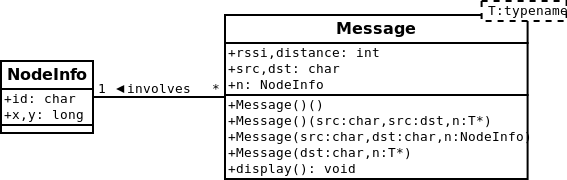
\includegraphics[width=0.5\textwidth]{msg.png}
\caption{Structure of a message}
\end{figure}
\noindent
\textbf{Q - Are there helpers structures?} \\
\textbf{A - }In order to run, the algorithm needs some information related to the node. However, the
structure is heavy to access and it is much more simple to keep the necessary information in another structure. This saves time but not memory. But
it avoids dynamic casts to access the desired information. The location algorithm runs with the following simplified structure of node.
\begin{figure}[H]
\centering
 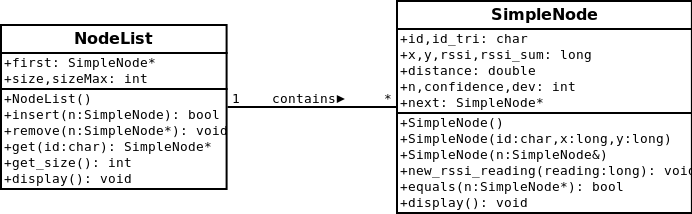
\includegraphics[width=0.5\textwidth]{simpleNode.png}
\caption{Simplified structure of a node}
\end{figure}
\noindent
\textbf{Q - How does HECOPS work?} \\
\textbf{A - }The simplest way to answer this question is to take a look at the following state machines.
\begin{figure}[H]
\centering
 \includegraphics[width=0.5\textwidth]{./anchor_behavior.png}
\caption{HECOPS state machine - behavior of an anchor node}
\end{figure}
\begin{figure}[H]
\centering
 \includegraphics[width=\textwidth]{./mobile_behavior.png}
\caption{HECOPS state machine - behavior of a mobile node}
\end{figure}
\noindent
Here is the pseudo-code on which is based the implementation of HECOPS@EPOS.
\begin{figure}[H]
\begin{algorithm}[H]
\caption{Pseudo-code for updating tables}
\begin{algorithmic}[H]
\IF{table is full}
\STATE replace line with less confidence
\ELSE 
\STATE include line in the table
\ENDIF
\FOR{line=first .. line $<=$ last}
\STATE read line
\STATE check if there is a tri formed by the 3 nodes: beacon, receiving and line n
\IF{tri==true AND $C_n > C_{min}$}
\STATE include or replace (if full) line in table
\ELSE
\STATE read next line
\ENDIF
\ENDFOR
\STATE select lines from table with top confidence
\IF{only one landmark}
\STATE assume position is (x,y+$d_{A,B}$)
\ELSE
\STATE calculate position (x,y)
\ENDIF
\STATE calculate confidence $C_b$ of nodes' position
\end{algorithmic}
\end{algorithm}
\caption{HECOPS algorithm}
\end{figure}
\noindent
\textbf{Q - Who can I contact if I have more questions?} \\
\textbf{A - }Thibault Rihet: \href{mailto:thibault@lisha.ufsc.br}{thibault@lisha.ufsc.br}
\begin{landscape}
\begin{figure}[H]
\centering
 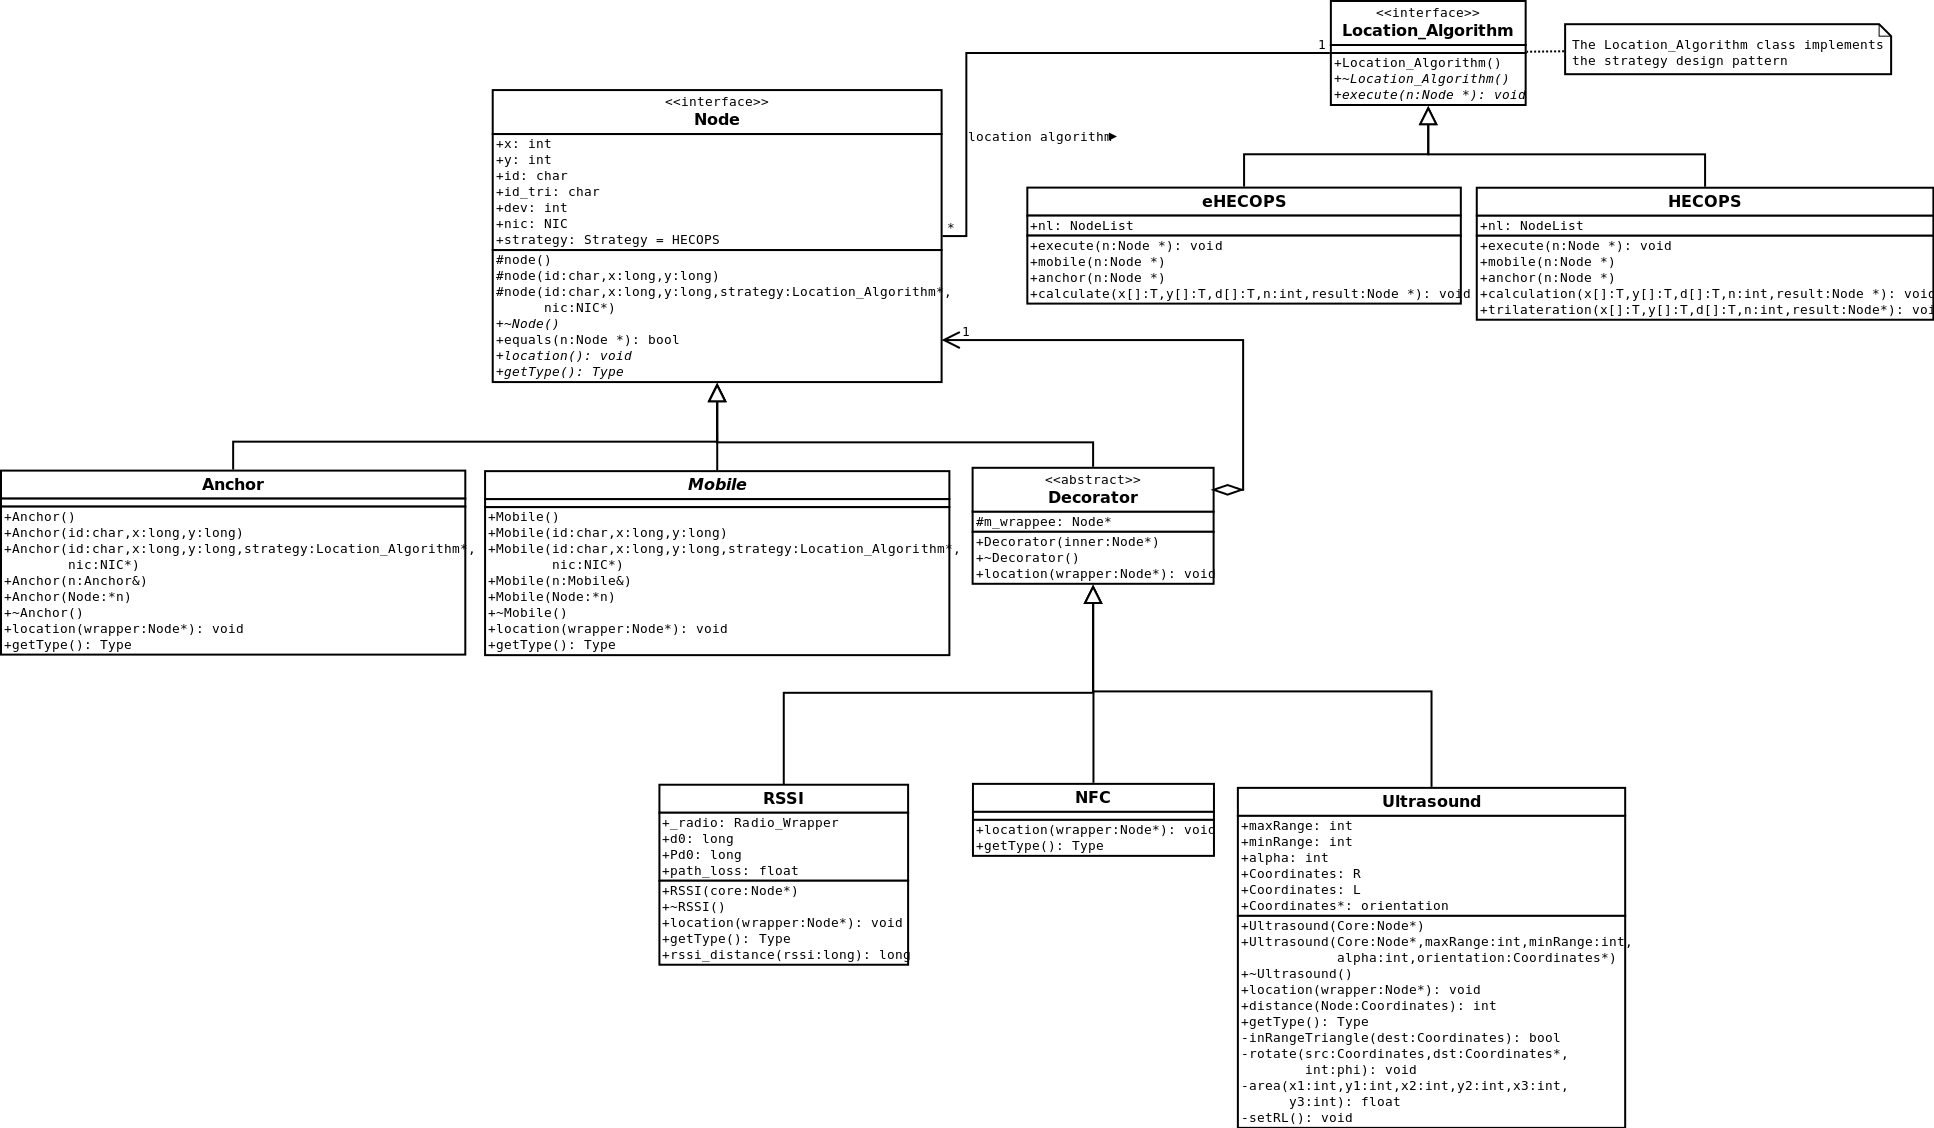
\includegraphics[width=1.5\textwidth]{./classdiagram.png}
\caption{Architecture of the localization algorithm for EPOS}
\end{figure}
\end{landscape}
\noindent 
Hereinunder are explained the main methods:\\ \\
\textbf{void Node::location()} \\
This method is the one called when a node wants to know its position. It applies the strategy that has been defined at its instanciation.\\ \\
\textbf{long RSSI::rssi\_distance(long rssi)}\\
This method estimates the distance between itself and the emitter of a message which signal was received with a strength of rssi. This method
uses the environment parameters that have been set up at the initialization of the object.\\ \\
\textbf{int Ultrasound::distance(Coordinates Node)}\\
This method attempts to estimate the distance between itself and another node of coordinates Node. If the node is not in the range triangle, it
returns -1; else, it emits an ultrasonic sound signal and attempts to measure the distance.\\ \\
\textbf{bool Ultrasound::inRangeTriangle(Coordinates dest)}\\
This method checks if a node is in its range triangle (cf. implementation section).\\ \\
\textbf{void Ultrasound::rotate(Coordinates src, Coordinates* dst, int phi)}\\
This method is a helper function that rotates the vector $\overrightarrow{the node, src}$ of an angle phi. The result is stored in dst.\\ \\
\textbf{float Ultrasound::area(int x1, int y1, int x2, int y2, int x3, int y3) }\\
This method is a helper function that calculates the area of a triangle formed by A(x1, y1), B(x2, y2) and C(x3, y3).\\ \\
\textbf{void Ultrasound::setRL() }\\
This method sets up the points R and L, edges of the range triangle.\\ \\
\textbf{void Location\_Algorithm::execute()} \\
This method executes the chosen strategy.\\ \\
\textbf{void HECOPS::mobile(Node* n)}\\
This method applies the behavior for a mobile.\\ \\
\textbf{void HECOPS::anchor(Node* n)}\\
This method applies the behavior for an anchor.\\ \\
\textbf{void HECOPS::trilateration(T x[], T y[], T d[], int n, Node* result)}\\
This method calculates the position of a node who has a list of n known positions and values of RSSI/distance estimation.

\end{document}
